\section{Bases de données moléculaires}
\label{donnees_bases}

\par Depuis une dizaine d'années, des bases de données contenant des millions de molécules ont émergé. Elles permettent aux chimistes d'avoir accès librement à une information riche décrivant la topologie, les différentes formules moléculaires ainsi que certaines propriétés basiques des molécules. La base la plus grande de ce genre, composée de molécules qui ont été synthétisées et étudiées, est la base de données Pubchem\cite{pubchem}, qui contient à ce jour plus de 90 millions de molécules. Elle offre également un système d'identification unique des molécules contenues (numéro CID). \\
Il existe également des bases de données composées de molécules théoriques issues de la combinaison d'éléments et respectant des règles simples permettant de vérifier qu'elles sont stables et synthétisables. Ces bases sont des sous-ensembles de l'univers GDB-17\cite{gdb}, énumérant 166 milliards de molécules dont le nombre d'atomes lourds (hors hydrogène) est inférieur ou égal à 17.\\

\par En plus des bases de données moléculaires, des bases de données de calculs quantiques ont été créées. Elles contiennent l'optimisation géométrique et les coefficients de la fonction d'onde des molécules, issus de calculs à grande échelle par des programmes de chimie informatique (\ref{opti_geom}). Parmi ces bases de données, on trouve notamment les bases QM7 et QM9, calculées sur des sous-ensembles de l'univers GDB-17, ainsi que la base PubchemQC\cite{pubchemqc}, calculée sur un sous-ensemble de Pubchem et composée d'environ quatre millions de molécules.\\

\par Dans le cadre de nos travaux, nous travaillons sur les molécules issues de la base PubchemQC. Ce choix est motivé par la plus grande hétérogénéité des molécules qui la composent, et va donc a priori permettre d'entraîner des modèles prédictifs qui se généraliseront mieux aux données des cas d'utilisation réels. La base de données que l'on utilise a été extraite des fichiers de sortie des logiciels de chimie informatique par Nicolas Roux lors de son stage en 2017. Pour chaque molécule, elle contient le numéro atomique et la masse atomique de chaque atome, ainsi que sa géométrie optimisée sous forme d'une matrice de coordonnées (\ref{repr_mat_coords}).

\section{Analyse des données}

\subsection{Distribution des tailles de molécules}

\label{donnees_distrib_tailles}

\par La base de données PubchemQC contient un certain nombre de calculs concernant des molécules que l'on ne peut pas utiliser pour des tâches d'optimisation géométrique. Elle contient en effet 26 molécules vides et 37 molécules contenant un seul atome. La présence de ces molécules dans les données d'apprentissage risque en effet d'induire les modèles en erreur.  Avant d'effectuer un nettoyage des données, nous nous intéressons à la distribution des tailles de molécules, visible dans la figure \ref{fig_distrib_tailles}. Il y apparaît que la taille des molécules suit une distribution gaussienne de centre 30. Dans le but de limiter la taille des entrées des modèles (\ref{dist_rel_homog_entrees}), nous allons également fixer une taille maximale aux molécules contenues dans le jeu de données nettoyé. Nous fixons cette limite à 60 atomes, afin que la quasi-totalité des molécules du jeu original soient conservées.\\
Tous les modèles décrits dans le chapitre \ref{dist_rel_chap} et certains modèles décrits dans le chapitre \ref{delta_dist_chap} (voir annexe \ref{annexes_param_delta_dist}) utilisent donc le jeu de données nettoyé contenant les molécules de tailles comprises entre 2 et 60.

\begin{figure}
	\centering
	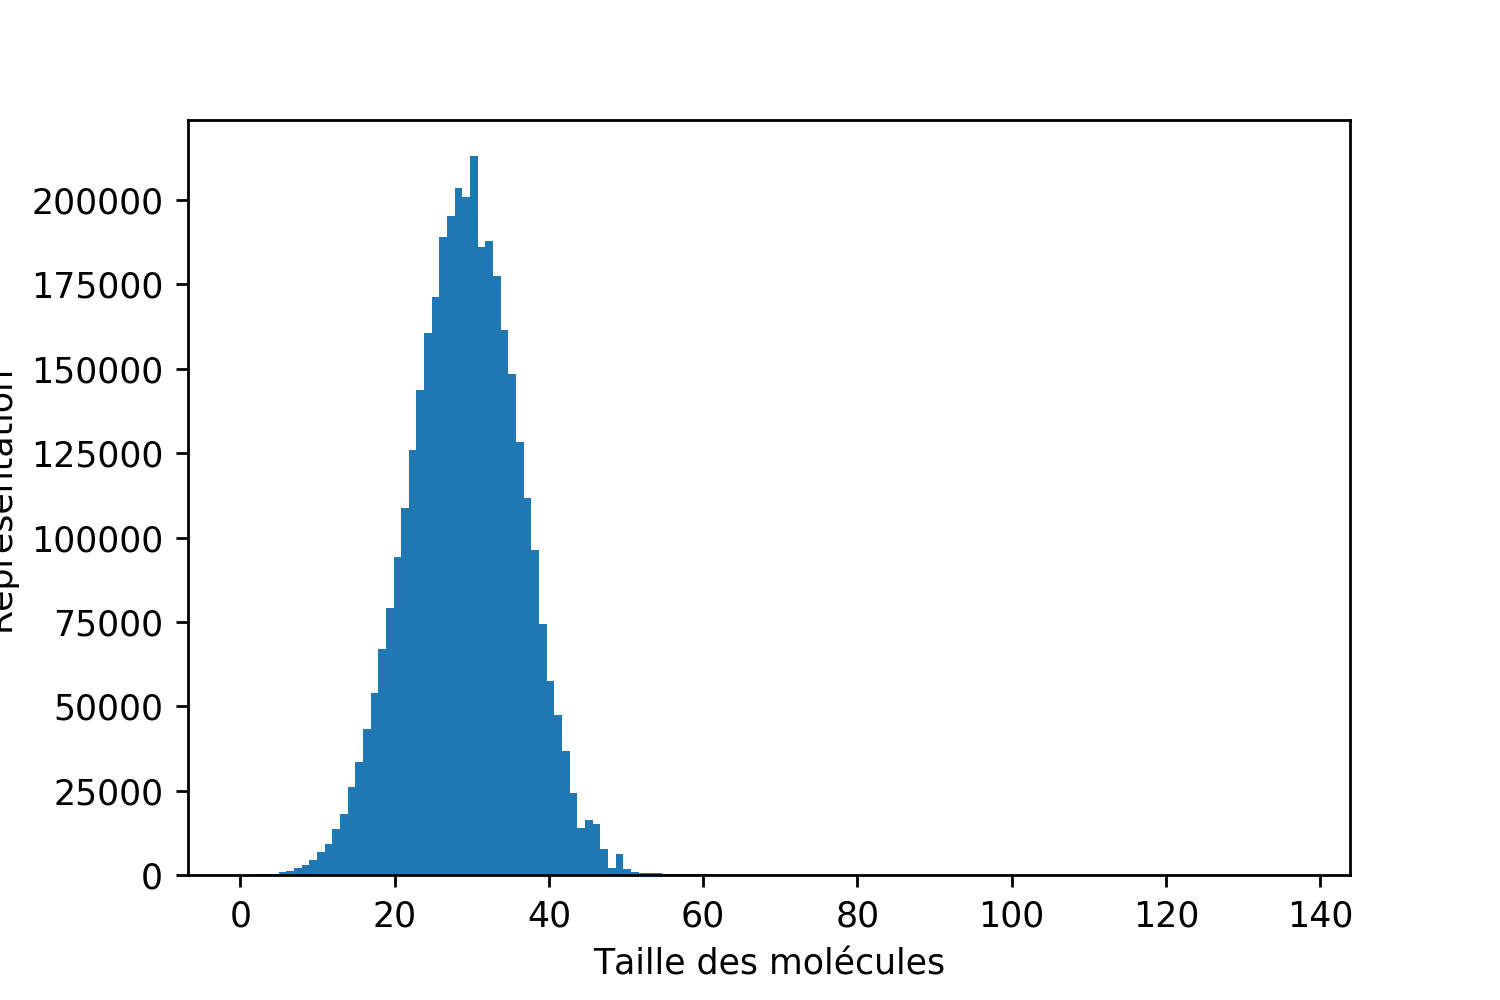
\includegraphics[scale=0.8]{../figures/80_distribution_molecules.png}
	\caption{Distribution des tailles de molécules dans les données de la base PubchemQC}
	\label{fig_distrib_tailles}
\end{figure}

\subsection{Distribution des longueurs de liaisons}

\label{donnees_distrib_longueurs_liaisons}


\par Afin de mieux comprendre les données sur lesquelles nous travaillons, et notamment dans le cas où l'on tente de prédire les longueurs de certains types de liaisons (chapitre \ref{dist_rel_chap}), nous étudions la distribution de la taille de ces différentes liaisons. Nous nous intéressons ici uniquement aux liaisons covalentes, c'est à dire aux couples d'atomes partageant au moins deux électrons. Les données que nous possédons n'indiquent pas quels sont les couples d'atomes qui partagent une liaison covalente. Par conséquent, nous déduisons cette information de la distance qui sépare les atomes de chaque couple, en utilisant l'étude de leurs distances types. Nous donnons dans le tableau \ref{table_dist_liaisons} les distances limites telles que l'on considère que deux atomes partagent une liaison covalentes. Ces distances sont données pour les trois couples d'atomes dont on prédit les longueurs de liaisons convergées.

\begin{table}
	\centering
	\begin{tabular}{|c|r|r|}
		\hline
		\textbf{Liaison} & \textbf{Distance minimale} & \textbf{Distance maximale} \\ \hline
		Carbone-carbone & 0 & 160 \\ \hline
		Carbone-hydrogène & 83 & 131 \\ \hline
		Oxygène-hydrogène & 90 & 125 \\ \hline
	\end{tabular}
	
	\caption{Longueurs telles que les couples d'atomes sont considérés comme partagent une liaison covalente (en pm)}
	\label{table_dist_liaisons}
\end{table}

\par Nous représentons graphiquement la distribution des longueurs de liaisons covalentes pour les trois couples d'atomes qui nous intéressent. On y remarque que la longueur des liaisons carbone-hydrogène (figure \ref{fdistrib_ch}) et oxygène-hydrogène (figure \ref{fdistrib_oh}) varie peu, mais que celle des liaisons carbone-carbone (figure \ref{fdistrib_cc}) prend une grande étendue de valeurs. Cela est lié aux multiples types de liaisons pouvant exister entre des atomes de carbone. Ces liaisons, qui dépendent du nombre d'électrons partagés, peuvent en effet être de type simple (154 pm), aromatique (140 pm), doubles (134 pm) ou triples (120 pm). La frontière entre les différents types de liaisons est en général continue, c'est pourquoi de nombreuses liaisons possèdent des tailles intermédiaires.

\begin{figure}
	\centering
	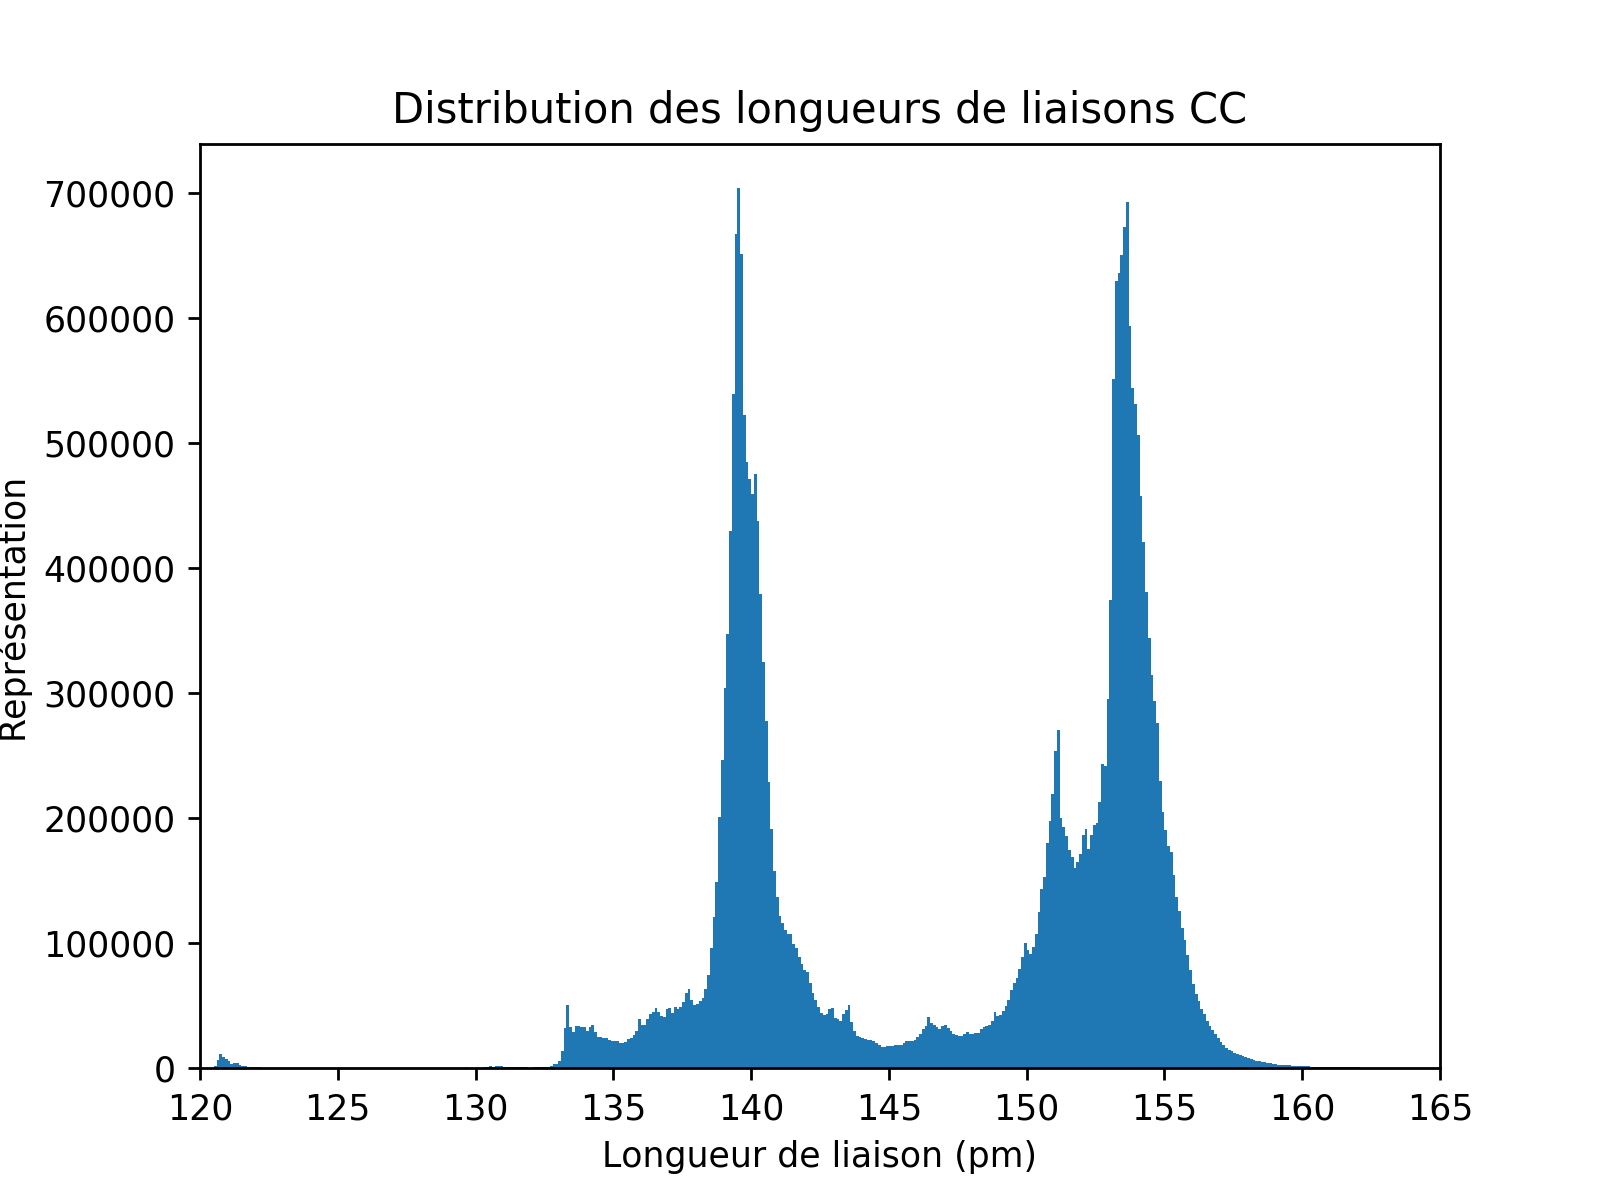
\includegraphics[scale=0.8]{../figures/distribCC.png}
	\caption{Distribution des longueurs de liaisons covalentes carbone-carbone}
	\label{fdistrib_cc}
\end{figure}

\begin{figure}
	\centering
	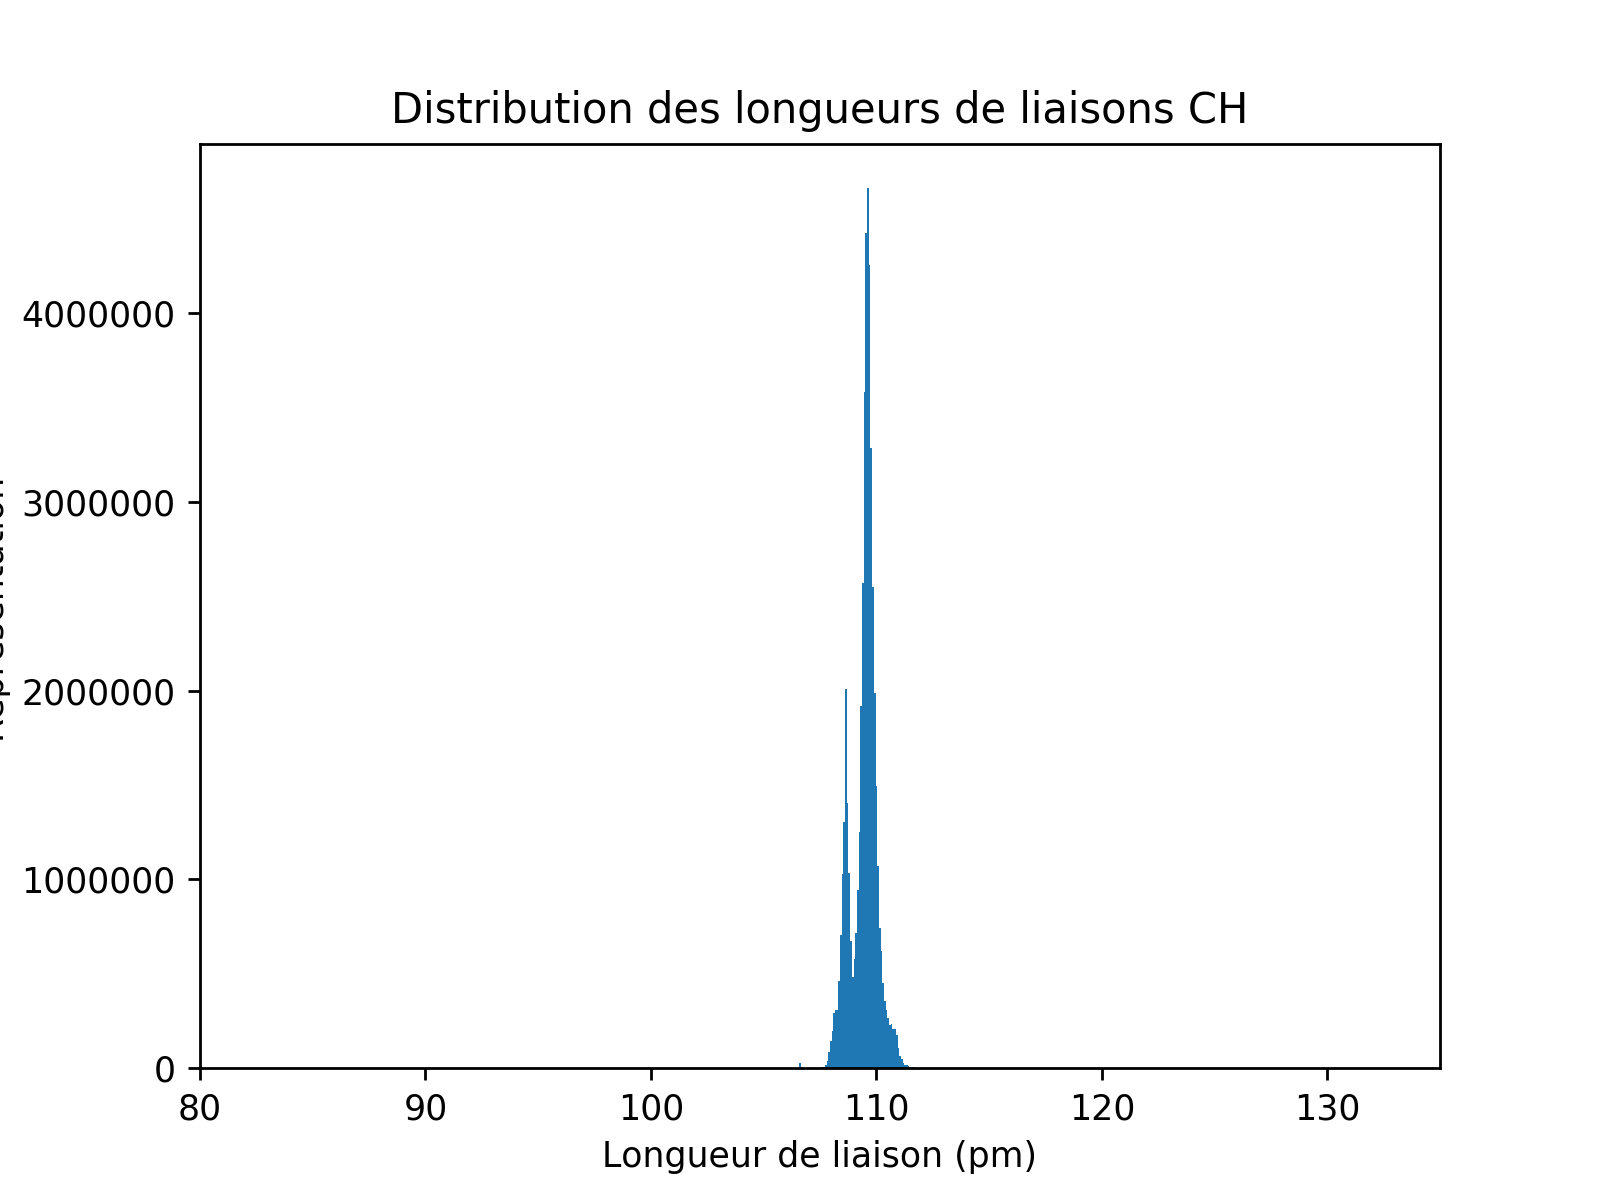
\includegraphics[scale=0.8]{../figures/distribCH.png}
	\caption{Distribution des longueurs de liaisons covalentes carbone-hydrogène}
	\label{fdistrib_ch}
\end{figure}

\begin{figure}
	\centering
	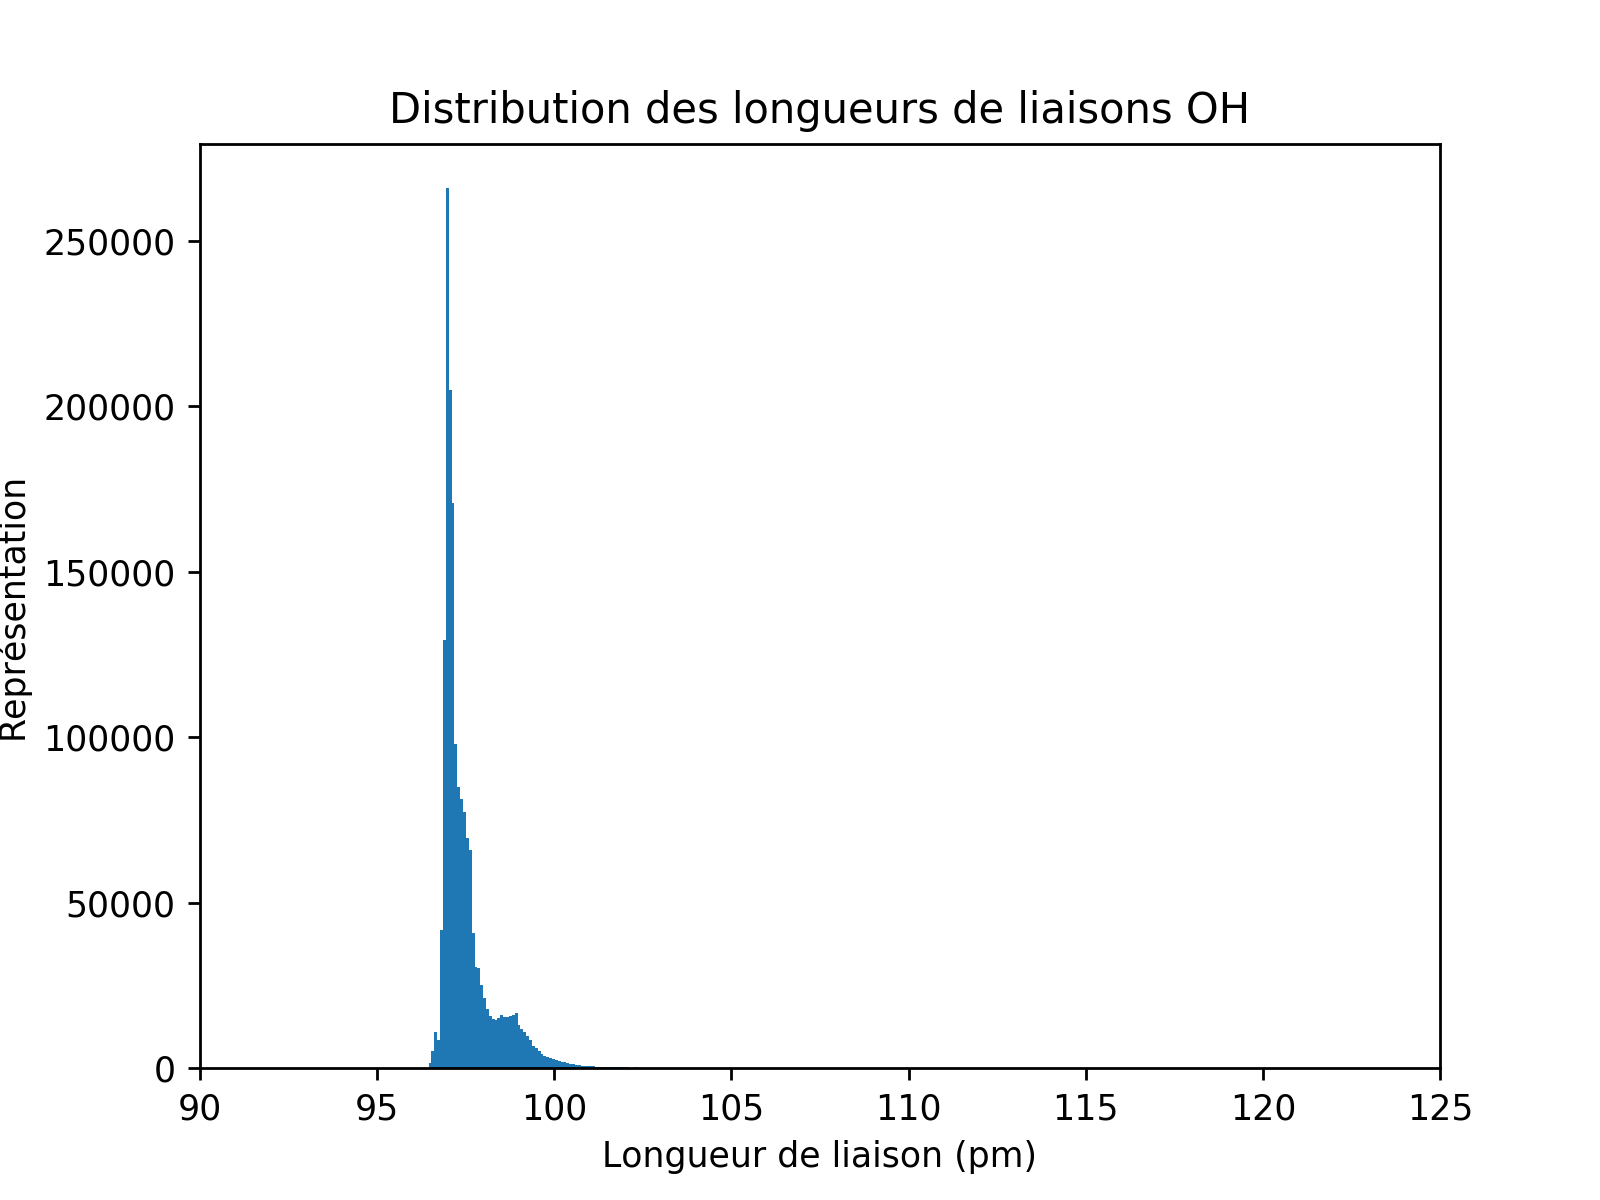
\includegraphics[scale=0.8]{../figures/distribOH.png}
	\caption{Distribution des longueurs de liaisons covalentes oxygène-hydrogène}
	\label{fdistrib_oh}
\end{figure}